    \section{TODO: Singular Value Decomposition}
    Unfortunately, as we know, not all matrices can be factored as $A = PDP^{-1}$ with $D$ diagonal. However, a factorization $A = QDP^{-1}$ is possible for \textit{any} $m\times n$ matrix $A$! A special factorization of this type, called the \textbf{singular value decomposition}, is \textbf{\textcolor{red}{the most useful matrix decomposition in the universe.}}\emoji{wink} \par
    If $A\B{x} = \lambda \B{x}$ and $\norm{\B{x}} = 1$, then
    \begin{equation*}
        \norm{A\B{x}} = \norm{\lambda \B{x}} = |\lambda| \norm{\B{x}} = |\lambda|
    \end{equation*} If $\lambda_1$ is the eigenvalue with the greatest magnitude, then a corresponding unit eigenvector $\B{v}_1$ identifies a direction in which the stretching effect of $A$ is greatest.

    \begin{Ex}
      If the linear transformation $\B{x}\to A\B{x}$ maps the unit sphere $\{ \B{x}: \norm{\B{x}} = 1 \}$ in $\R^3$ onto an ellipse in $\R^2$. Find a unit vector $\B{x}$ at which the length $\norm{A\B{x}}$ is maximized, and compute this maximum length.
      \begin{sol}
          The quantity $\norm{A\B{x}}^2$ is maximized at the same $\B{x}$ that maximizes $\norm{A\B{x}}$, 
          \begin{equation*}
              \norm{A\B{x}}^2 = \T{(A\B{x})}(A\B{x}) = \T{\B{x}}(\T{A}A)\B{x}
          \end{equation*} Since $\T{A}A$ is symmetric, so the problem is reduced into maximizing the quadratic form $\T{\B{x}}(\T{A}A)\B{x}$ subject to the constraint $\norm{\B{x}} = 1$ as discussed in \cref{unit-opt}. Hence, the maximum value is the greatest eigenvalue $\lambda_1$ of $\T{A}A$, and the maximum value is attained at a unit eigenvector of $\T{A}A$ corresponding to $\lambda_1$.
      \end{sol}
    \end{Ex}
    The example above suggests that the effect of $A$ on the unit sphere in $\R^3$ is related to the quadratic form $\T{x}(\T{A}A)\B{x}$.\par 
    Let $A\in\R^{m\times n}$. Then $\T{A}A$ can be orthogonally diagonalized. Let $\{\B{v}_1, \cdots, \B{v}_n \}$ be an orthonormal basis for $\R^n$ consisting of eigenvectors of $\T{A}A$. Then,
    \begin{equation}\label{t}
        \norm{A\B{v}_i} = \T{(A\B{v}_i)}A\B{v}_i = \T{\B{v}_i}(\lambda_i \B{v}_i) = \lambda_i\geq 0
    \end{equation}Note that $\norm{\B{v}_i} = 1$. So \textbf{\textcolor{orange}{the eigenvalues of $\T{A}A$ are all non-negative, implying that $\T{A}A$ is a semi-positive definite matrix.}}
    \begin{Def}
        The singular values of $A$ are the square roots of the eigenvalues of $\T{A}A$, denoted by $\sigma_1, \cdots, \sigma_n$, and they are arranged in decreasing order. By \cref{t}, the \textbf{singular values of $A$ are the lengths of the vectors $A\B{v}_1, \cdots, A\B{v}_n$}. 
        \begin{Rem}
            The first two singular values of $A$ are the lengths of the major and minor semi-axes of the ellipse as shown \cref{singular-ellipse}.
        \end{Rem}
    \end{Def}
    \begin{figure}
        \centering
        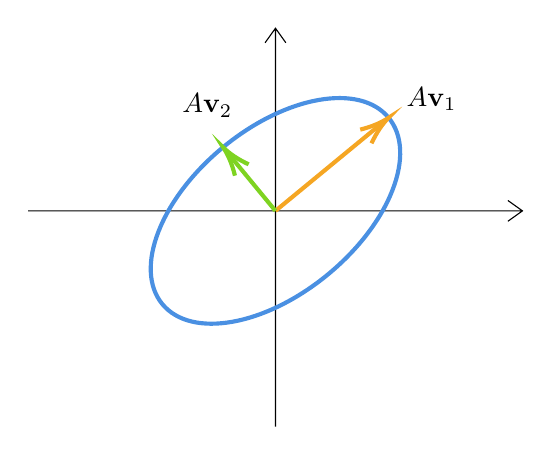
\begin{tikzpicture}[x=0.75pt,y=0.75pt,yscale=-1,xscale=1]
%uncomment if require: \path (0,300); %set diagram left start at 0, and has height of 300

%Shape: Axis 2D [id:dp5842664307886825] 
\draw  (216,137) -- (454.11,137)(335.11,49) -- (335.11,241) (447.11,132) -- (454.11,137) -- (447.11,142) (330.11,56) -- (335.11,49) -- (340.11,56)  ;
%Shape: Ellipse [id:dp9660000625734635] 
\draw  [color={rgb, 255:red, 74; green, 144; blue, 226 }  ,draw opacity=1 ][line width=1.5]  (280.59,181.88) .. controls (266.65,164.95) and (279.76,131.13) .. (309.87,106.34) .. controls (339.99,81.55) and (375.7,75.18) .. (389.64,92.12) .. controls (403.58,109.05) and (390.46,142.87) .. (360.35,167.66) .. controls (330.24,192.45) and (294.52,198.82) .. (280.59,181.88) -- cycle ;
%Straight Lines [id:da36332977734700256] 
\draw [color={rgb, 255:red, 245; green, 166; blue, 35 }  ,draw opacity=1 ][line width=1.5]    (335.11,137) -- (387.32,94.02) ;
\draw [shift={(389.64,92.12)}, rotate = 140.54] [color={rgb, 255:red, 245; green, 166; blue, 35 }  ,draw opacity=1 ][line width=1.5]    (14.21,-4.28) .. controls (9.04,-1.82) and (4.3,-0.39) .. (0,0) .. controls (4.3,0.39) and (9.04,1.82) .. (14.21,4.28)   ;
%Straight Lines [id:da7831499075107744] 
\draw [color={rgb, 255:red, 126; green, 211; blue, 33 }  ,draw opacity=1 ][line width=1.5]    (335.11,137) -- (311.78,108.65) ;
\draw [shift={(309.87,106.34)}, rotate = 50.54] [color={rgb, 255:red, 126; green, 211; blue, 33 }  ,draw opacity=1 ][line width=1.5]    (14.21,-4.28) .. controls (9.04,-1.82) and (4.3,-0.39) .. (0,0) .. controls (4.3,0.39) and (9.04,1.82) .. (14.21,4.28)   ;

% Text Node
\draw (397,76.4) node [anchor=north west][inner sep=0.75pt]    {$A\mathbf{v}_{1}$};
% Text Node
\draw (289,79.4) node [anchor=north west][inner sep=0.75pt]    {$A\mathbf{v}_{2}$};


\end{tikzpicture}
        \caption{$A\B{v}_1$ is the major semi-axis and $A\B{v}_2$ is the minor semi-axis of the ellipse.}
        \label{singular-ellipse}
    \end{figure}

    \begin{Thm}\label{t-1}
        Suppose $\{\B{v}_1, \cdots, \B{v}_n\}$ is an orthonormal basis of $\Rn$ consisting of eigenvectors of $\T{A}A$, arranged so that the corresponding eigenvalues of $\T{A}A$ satisfy $\lambda_1\geq \cdots\geq \lambda_n$, and suppose that $A$ has $r$ nonzero singular values. Then $\{A\B{v}_1, \cdots, A\B{v}_r \}$ is an orthogonal basis for $\text{Col}(A)$, and $\text{rank}(A) = r$.
        \begin{proof}
            Given two vectors $A\B{v}_j, A\B{v}_i$ where $i\neq j$, 
            \begin{equation*}
                \T{(A\B{v}_j)}A\B{v}_i = \T{\B{v}_j}\T{A}A\B{v}_i = \lambda_i \T{\B{v}_j}\B{v}_i = 0 
            \end{equation*} Thus, $\{A\B{v}_1, \cdots, A\B{v}_n \}$ is an orthogonal set. Furthermore, since the lengths of the vector $\{A\B{v}_1, \cdots, A\B{v}_n$ are the singular values of $A$, and since there are $r$ non-zero singular values, $A\B{v}_i\neq \B{0}$ if and only if $1\leq i\leq r$. So, $\{A\B{v}_1, \cdots, A\B{v}_r$ are linearly independent vectors, and they are in $\text{Col}(A)$. $\forall \B{y}\in\text{Col}(A)$, say $\B{y} = A\B{x}$ , we can write
            \begin{equation*}
                \B{x} = c_1\B{v}_1 + \cdots + c_n\B{v}_n
            \end{equation*}, and 
            \begin{align*}
                \B{y} &= A\B{x}\\
                & = c_1A\B{v}_1 + \cdots + c_rA\B{v}_r + c_{r+1}A\B{v}_{r+1} + \cdots + c_nA\B{v}_n\\
                & = c_1A\B{v}_1 + \cdots + c_rA\B{v}_r + 0 + 0 + \cdots + 0
            \end{align*} Thus $\B{y}$ is in $\text{Span}\{A\B{v}_1, \cdots, A\B{v}_r \}$, which shows that $\{ A\B{v}_1, \cdots, A\B{v}_r \}$ is an (orthogonal) basis for $\text{Col}(A)$. Hence $\text{rank}(A) = \text{dim}\Big(\text{Col}(A)\Big) = r$.
        \end{proof}
    \end{Thm}
The decomposition of $A$ involves an $m\times n$ \enquote{diagonal} matrix $\Lambda$ of the form
\begin{equation}\label{Lambda}
    \Lambda = \begin{bmatrix}
        D & \B{O}\\
        \B{O} & \B{O}
    \end{bmatrix}
\end{equation} where $D$ is an $r\times r$ diagonal matrix for some $r$ not exceeding the smaller of $m$ and $n$.

\begin{Thm}
    \textbf{The Singular Value Decomposition or (SVD)}: 
    Let $A$ be an $m\times n$ matrix with rank $r$. then there exists an $m\times n$ matrix $\Lambda$ as in \cref{Lambda} for which the diagonal entries in $D$ are the first singular values of $A$, $\sigma_1\geq \sigma_2\geq \cdots \geq \sigma_r\geq 0$, and there exist an $m\times n$ orthogonal matrix $U$ and an $n\times n$ orthogonal matrix $V$ such that
    \begin{equation*}
        A = U\Lambda \T{V}
    \end{equation*}
    \begin{proof}
        Let $\lambda_i$ and $\B{v}_i$ be as in \cref{t-1}, so that $\{A\B{v}_1, \cdots, A\B{v}_r \}$ is an orthogonal basis for $\text{Col}(A)$. Normalize each $A\B{v}_i$ to obtain an orthonormal basis $\mathcal{U} = \{\B{u}_1, \cdots, \B{u}_r \}$, where
        \begin{equation}
            \B{u}_i = \cfrac{A\B{v}_i}{\norm{A\B{v}_i}} = \cfrac{A\B{v}_i}{\sigma_i}
        \end{equation} and 
        \begin{equation}
            A\B{v}_i = \sigma_i \B{u}_i
        \end{equation} Now extend $\mathcal{U}$ to an orthonormal basis $\{ 
\B{u}_1, \cdots, \B{u}_m \}$ of $\R^m$, and let 
        \begin{equation}
            U = \begin{bmatrix}
                \B{u_1} & \cdots & \B{u}_m
            \end{bmatrix} \quad \text{and }\quad \begin{bmatrix}
                    \B{v}_1 & \cdots & \B{v}_n
                \end{bmatrix}
        \end{equation} By construction, $U$ and $V$ are orthogonal matrices. Also,
        \begin{equation}
            AV = \begin{bmatrix}
                A\B{v}_1 & \cdots & A\B{v}_r & \B{0} & \cdots & \B{0} 
            \end{bmatrix} = \begin{bmatrix}
                    \sigma_1\B{u}_1 & \cdots & \sigma_r\B{u}_r & \B{0} & \cdots & \B{0}
                \end{bmatrix}
        \end{equation} Let $D$ be the diagonal matrix with diagonal entries $\sigma_1,\cdots, \sigma_r$, and let $\Lambda$ be as in \cref{t-1} above. Then
        \begin{equation}
            U\Lambda = \begin{bmatrix}
                U_1 & U_2
            \end{bmatrix} \begin{bmatrix}
                    D & \B{O}\\
                    \B{O} & \B{O}
                \end{bmatrix} = \begin{bmatrix}
                    U_1 D & \B{O}
                \end{bmatrix} = AV
        \end{equation}
        where $U_1 = \begin{bmatrix}
            \B{u}_1 & \cdots & \B{u}_r
        \end{bmatrix}$ and $U_2 = \begin{bmatrix}
            \B{u}_{r+1} & \cdots & \B{u}_{m}
        \end{bmatrix}$. Since $V$ is an orthogonal matrix,
        \begin{equation*}
            U\Lambda \T{V} = AV\T{V} = A
        \end{equation*}
    \end{proof}
    \begin{Rem}
            The columns of $U$ are called \textbf{left singular vectors} of $A$, and the columns of $V$ are called \textbf{right singular vectors} of $A$.
    \end{Rem}
\end{Thm}
\subsection{Bases for Fundamental Subspaces}
Given an SVD decomposition for a $m\times n$ matrix $A$, by observing its left singular vectors, we can find that $\{\B{u}_1, \cdots, \B{u}_r \}$ is an orthonormal basis for $\text{Col}(A)$ by \cref{t-1}, and $\{\B{u}_{r+1}, \cdots, \B{u}_n\}$ is an orthonormal basis for $\text{Nul}(\T{A})$, since for any $r< i\leq n$, $\B{u}_i$ is orthogonal to $\text{Col}(A) = \text{Span}\{\B{u}_1, \cdots, \B{u}_{r} \}$, that is, $\text{Span}\{\B{u}_{r+1}, \cdots, \B{u}_m \} = \text{Col}(A)^\perp$.\par
    Since $\{\B{u}_1, \cdots, \B{u}_r \}$ forms a basis for $\text{Col}(A)$, $\text{dim}(A) = r$, implying $\text{dim}\Big(\text{Nul}(A) \Big) = n - r$. For any $i > r$, since $A\B{v}_i = \B{0}$ and $\text{dim}\Big(\text{Nul}(A) \Big) = n - r$, $\text{Span}\{\B{v}_{r+1}, \cdots, \B{v}_{n} \} = \text{Nul}(A)$. Note that $\text{Nul}(A)^\perp = \text{Row}(A)$. Hence, $\{\B{v}_1,\cdots, v_r \}$ is an orthonormal basis for $\text{Row}(A)$. Observing that
    \begin{equation*}
        AV = \begin{bmatrix}
                A\B{v}_1 & \cdots & A\B{v}_r & \B{0} & \cdots & \B{0} 
            \end{bmatrix} = \begin{bmatrix}
                    \sigma_1\B{u}_1 & \cdots & \sigma_r\B{u}_r & \B{0} & \cdots & \B{0}
                \end{bmatrix}
    \end{equation*} for which the non-zero vectors of $AV$ is an orthogonal basis for $\text{Col}(A)$. In other words, the matrix $A$ transforms a collection of basis vectors of $\text{Col}(A)$ and $\text{Nul}(\T{A})$ into a collection of basis of $\text{Row}(A)$ and $\text{Nul}(A)$. 
    
    Let $V = \begin{bmatrix}
        \B{v}_1 & \cdots & \B{v}_r
    \end{bmatrix}$, $\begin{bmatrix}
        \B{v}_{r+1} & \cdots & \B{v}_{n}
    \end{bmatrix}$. And let $U_1 = \begin{bmatrix}
        \B{u}_1 & \cdots & \B{u}_r
    \end{bmatrix}$, $\begin{bmatrix}
        \B{u}_{r+1} & \cdots & \B{u}_{m}
    \end{bmatrix}$, they have the relationship shown as \cref{SVD-relation},
    \begin{figure}
        \centering
        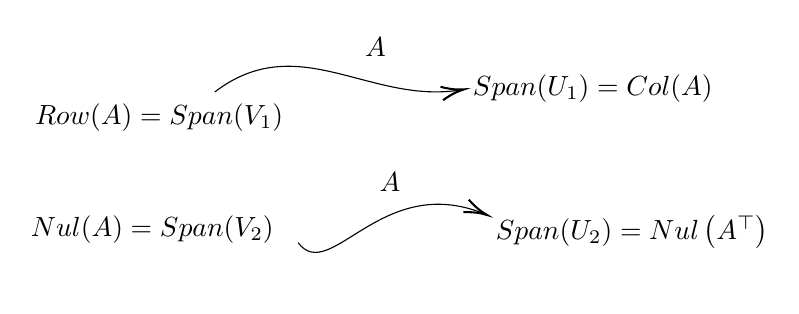
\begin{tikzpicture}[x=0.75pt,y=0.75pt,yscale=-1,xscale=1]
%uncomment if require: \path (0,300); %set diagram left start at 0, and has height of 300


% Text Node
\draw (278,88.4) node [anchor=north west][inner sep=0.75pt]    {$\text{Span}(U_{1}) =\text{Col}(A)$};
% Text Node
\draw (289,156.4) node [anchor=north west][inner sep=0.75pt]    {$\text{Span}(U_{2}) =\text{Nul}\left( A^{\top }\right)$};
% Text Node
\draw (67,102.4) node [anchor=north west][inner sep=0.75pt]    {$\text{Row}(A) =\text{Span}(V_{1})$};
% Text Node
\draw (65,156.4) node [anchor=north west][inner sep=0.75pt]    {$\text{Nul}(A)=\text{Span}(V_{2})$};
% Text Node
\draw (226,70.4) node [anchor=north west][inner sep=0.75pt]    {$A$};
% Text Node
\draw (233,135.4) node [anchor=north west][inner sep=0.75pt]    {$A$};
% Connection
\draw    (195,170.6) .. controls (210.41,191.15) and (235,136.53) .. (284.49,156.63) ;
\draw [shift={(286,157.26)}, rotate = 203.39] [color={rgb, 255:red, 0; green, 0; blue, 0 }  ][line width=0.75]    (10.93,-3.29) .. controls (6.95,-1.4) and (3.31,-0.3) .. (0,0) .. controls (3.31,0.3) and (6.95,1.4) .. (10.93,3.29)   ;
% Connection
\draw    (154.9,98) .. controls (195.13,67.3) and (229.57,104.33) .. (273.66,96.98) ;
\draw [shift={(275,96.74)}, rotate = 169.44] [color={rgb, 255:red, 0; green, 0; blue, 0 }  ][line width=0.75]    (10.93,-3.29) .. controls (6.95,-1.4) and (3.31,-0.3) .. (0,0) .. controls (3.31,0.3) and (6.95,1.4) .. (10.93,3.29)   ;

\end{tikzpicture}
        \caption{The effect of $A$ on $V$.}
        \label{SVD-relation}
    \end{figure}